\documentclass{article}\usepackage[]{graphicx}\usepackage[]{color}
%% maxwidth is the original width if it is less than linewidth
%% otherwise use linewidth (to make sure the graphics do not exceed the margin)
\makeatletter
\def\maxwidth{ %
  \ifdim\Gin@nat@width>\linewidth
    \linewidth
  \else
    \Gin@nat@width
  \fi
}
\makeatother

\definecolor{fgcolor}{rgb}{0.345, 0.345, 0.345}
\newcommand{\hlnum}[1]{\textcolor[rgb]{0.686,0.059,0.569}{#1}}%
\newcommand{\hlstr}[1]{\textcolor[rgb]{0.192,0.494,0.8}{#1}}%
\newcommand{\hlcom}[1]{\textcolor[rgb]{0.678,0.584,0.686}{\textit{#1}}}%
\newcommand{\hlopt}[1]{\textcolor[rgb]{0,0,0}{#1}}%
\newcommand{\hlstd}[1]{\textcolor[rgb]{0.345,0.345,0.345}{#1}}%
\newcommand{\hlkwa}[1]{\textcolor[rgb]{0.161,0.373,0.58}{\textbf{#1}}}%
\newcommand{\hlkwb}[1]{\textcolor[rgb]{0.69,0.353,0.396}{#1}}%
\newcommand{\hlkwc}[1]{\textcolor[rgb]{0.333,0.667,0.333}{#1}}%
\newcommand{\hlkwd}[1]{\textcolor[rgb]{0.737,0.353,0.396}{\textbf{#1}}}%

\usepackage{framed}
\makeatletter
\newenvironment{kframe}{%
 \def\at@end@of@kframe{}%
 \ifinner\ifhmode%
  \def\at@end@of@kframe{\end{minipage}}%
  \begin{minipage}{\columnwidth}%
 \fi\fi%
 \def\FrameCommand##1{\hskip\@totalleftmargin \hskip-\fboxsep
 \colorbox{shadecolor}{##1}\hskip-\fboxsep
     % There is no \\@totalrightmargin, so:
     \hskip-\linewidth \hskip-\@totalleftmargin \hskip\columnwidth}%
 \MakeFramed {\advance\hsize-\width
   \@totalleftmargin\z@ \linewidth\hsize
   \@setminipage}}%
 {\par\unskip\endMakeFramed%
 \at@end@of@kframe}
\makeatother

\definecolor{shadecolor}{rgb}{.97, .97, .97}
\definecolor{messagecolor}{rgb}{0, 0, 0}
\definecolor{warningcolor}{rgb}{1, 0, 1}
\definecolor{errorcolor}{rgb}{1, 0, 0}
\newenvironment{knitrout}{}{} % an empty environment to be redefined in TeX

\usepackage{alltt}
\setlength{\topmargin}{-.5in}
\setlength{\textheight}{9in}
\setlength{\oddsidemargin}{.125in}
\setlength{\textwidth}{6.25in}

% comment

\usepackage{graphicx}
\usepackage{amsmath}
\DeclareGraphicsExtensions{.png,.jpg}

\title{Applied Data Science HW2}
\author{Xiaoyao Yang\\ Columbia University}
\date{\today}
\IfFileExists{upquote.sty}{\usepackage{upquote}}{}

\begin{document}
\maketitle

\section{Sergei’s problem}
\label{sec:q1}

\subsection{Categorical Variables with few level}
\label{q1-1}

First, we read data set using read.table function. And then we use For loop as well as model.matrix function to transfer Categorical Variables with limited level to Dummy Matrix. Noted that we only use for loop here one time and use model.matrix for other variables.

\begin{knitrout}
\definecolor{shadecolor}{rgb}{0.969, 0.969, 0.969}\color{fgcolor}\begin{kframe}
\begin{alltt}
\hlstd{dat} \hlkwb{=} \hlkwd{read.table}\hlstd{(}\hlstr{"columbia_data_set.csv"}\hlstd{,} \hlkwc{sep} \hlstd{=} \hlstr{","}\hlstd{,} \hlkwc{header} \hlstd{= T)}
\hlstd{n} \hlkwb{<-} \hlkwd{dim}\hlstd{(dat)[}\hlnum{1}\hlstd{]}
\hlstd{hour} \hlkwb{<-} \hlstd{dat}\hlopt{$}\hlstd{hour}
\hlstd{I_hour} \hlkwb{<-} \hlkwd{matrix}\hlstd{(}\hlnum{0}\hlstd{,} \hlkwc{nrow} \hlstd{= n,} \hlkwc{ncol} \hlstd{=} \hlnum{24}\hlstd{)}
\hlkwa{for} \hlstd{(i} \hlkwa{in} \hlnum{1}\hlopt{:}\hlstd{n) \{}
    \hlstd{I_hour[i, hour[i]]} \hlkwb{<-} \hlnum{1}
\hlstd{\}}
\hlcom{# hour<-as.factor(dat$hour) model.matrix(~hour-1)->a}

\hlcom{### state}
\hlstd{state} \hlkwb{<-} \hlkwd{as.factor}\hlstd{(dat}\hlopt{$}\hlstd{state)}
\hlstd{dummy_state} \hlkwb{<-} \hlkwd{model.matrix}\hlstd{(}\hlopt{~}\hlstd{state} \hlopt{-} \hlnum{1}\hlstd{)}
\hlcom{### browser.id}
\hlstd{browser.id} \hlkwb{<-} \hlkwd{as.factor}\hlstd{(dat}\hlopt{$}\hlstd{browser.id)}
\hlstd{dummy_browser.id} \hlkwb{<-} \hlkwd{model.matrix}\hlstd{(}\hlopt{~}\hlstd{browser.id} \hlopt{-} \hlnum{1}\hlstd{)}
\hlcom{### ad.size}
\hlstd{ad.size} \hlkwb{<-} \hlkwd{as.factor}\hlstd{(dat}\hlopt{$}\hlstd{ad.size)}
\hlstd{dummy_ad.size} \hlkwb{<-} \hlkwd{model.matrix}\hlstd{(}\hlopt{~}\hlstd{ad.size} \hlopt{-} \hlnum{1}\hlstd{)}
\hlcom{### ad.size}
\hlstd{ad.size} \hlkwb{<-} \hlkwd{as.factor}\hlstd{(dat}\hlopt{$}\hlstd{ad.size)}
\hlstd{dummy_ad.size} \hlkwb{<-} \hlkwd{model.matrix}\hlstd{(}\hlopt{~}\hlstd{ad.size} \hlopt{-} \hlnum{1}\hlstd{)}
\end{alltt}
\end{kframe}
\end{knitrout}


And we can take a look at first several rows of our Dummy Set

\begin{knitrout}
\definecolor{shadecolor}{rgb}{0.969, 0.969, 0.969}\color{fgcolor}\begin{kframe}
\begin{alltt}
\hlkwd{head}\hlstd{(dummy_ad.size)}
\end{alltt}
\begin{verbatim}
##   ad.size160x600 ad.size300x250 ad.size728x90
## 1              0              1             0
## 2              1              0             0
## 3              0              1             0
## 4              1              0             0
## 5              0              0             1
## 6              0              1             0
\end{verbatim}
\end{kframe}
\end{knitrout}


If we want to combined these Dummy Matrix. We can use cbind() function to do it.

\subsection{Site.id}
\label{q1-2}

 

\begin{knitrout}
\definecolor{shadecolor}{rgb}{0.969, 0.969, 0.969}\color{fgcolor}\begin{kframe}
\begin{alltt}
\hlkwd{table}\hlstd{(dat}\hlopt{$}\hlstd{site.id)}
\end{alltt}
\begin{verbatim}
## 
##     1     2     3     4     5     6     8     9    10    11    12    13 
##   185    99    44    12    21    14   133    48     1     6     3    34 
##    14    15    16    17    18    19    20    22    23    24    26    27 
##     9     1   201     1     1   175    35    83     1     3    10   175 
##    30    31    32    33    34    35    36    37    38    39    40    41 
##    16    37  1826    19   358    81    58  1109    14     4     9     9 
##    42    43    44    47    48    49    50    51    52    53    54    55 
##    55    67   368    69    55   403    29    14    25    57   158   477 
##    56    57    58    59    61    62    63    64    66    67    68    69 
##    55     1    11     1    32 45851    35    15     2     5     7   199 
##    70    71    72    73    74    75    76    77    78    79    80    81 
##    26   151   118     6    18     4    22   715   129     1    98    11 
##    82    83    84    85    86    87    88    89    90    91    92    93 
##     8    30    37     6   384    58     8   147    17     5    38     3 
##    95    99   100   101   102   103   104   105   107   108   109   110 
##    10    10     6   156  4121    30     2    23    68     2    10     1 
##   111   112   113   115   116   119   120   122   124   126   127   128 
##    32    10    60     5    31    71  5780    79     1  1394    92     2 
##   131   132   133   134   135   136   137   138   139   140   142   143 
##    40   100    89     3    12    14    31   126    64    39   104   121 
##   144   145   146   147   148   149   150   151   152   153   154   155 
##    28     1    46    37    23    16     7    32    12    50    36    55 
##   156   157   158   159   161   162   163   164   165   166   167   168 
##    14   123     1    18     3    26   189     3    14     1    18     6 
##   169   170   172   173   174   175   176   177   178   179   180   181 
##     1     3    51     5    38    30     2    72    14    44     4   171 
##   182   183   184   185   186   187   188   189   190   191   192   193 
##    16    30     3    97   293    33   462 11365    23   868    11  1328 
##   194   195   198   199   200   202   203   204   205   206   207   209 
##    32    40   492   103   369    31    52    81   184    81    20    10 
##   210   211   212   213   214   215   217   218   219   220   221   222 
##    34   121    69    14    15  1598     4    23    76   879   303   804 
##   223   224   225   229   231   232   233   234   236   237   238   242 
##     1    82  2151     2    17   399     1    23    29    26     2     1 
##   244   246   247   248   249   250   252   253   254   255   256   257 
##    41     4    43  1430     9   216     3    12     4    16     1   306 
##   259   260   261   262   264   266   267   268   269   270   271   272 
##   135     2    60     1     9   325   291    11    44   109    21     4 
##   273   274   275   276   277   278   279   280   281   282   283   284 
##    48     4     5    30    12   366    57    90   307    64    24    24 
##   285   286   287   288   289   290   291   295   296   297   298   299 
##   184   632    89  3376     3     1     2     1    24     1    34     3 
##   301   302   303   306   307   308   310 
##     1     3     4     3     2     9     3
\end{verbatim}
\end{kframe}
\end{knitrout}

From the table above we can see that there are too many different site.id. Thus, we pick up most frequent id and put other id in one column.

As a result, there is 256 different level for site.id variable. After simulate the cumulative density function, we finally collect 136 variables from 256 and put the rest variable into ``Other'' column.


\begin{knitrout}
\definecolor{shadecolor}{rgb}{0.969, 0.969, 0.969}\color{fgcolor}\begin{kframe}
\begin{alltt}
\hlcom{### site.id}
\hlstd{site} \hlkwb{<-} \hlstd{dat}\hlopt{$}\hlstd{site.id}
\hlstd{site.t} \hlkwb{<-} \hlkwd{table}\hlstd{(site)}
\hlstd{temp} \hlkwb{<-} \hlkwd{sort}\hlstd{(site.t,} \hlkwc{decreasing} \hlstd{=} \hlnum{TRUE}\hlstd{)}
\hlstd{site.cdf} \hlkwb{<-} \hlkwd{cumsum}\hlstd{(temp)}\hlopt{/}\hlkwd{sum}\hlstd{(temp)}
\hlstd{site.names} \hlkwb{<-} \hlkwd{names}\hlstd{(temp)[site.cdf} \hlopt{<} \hlnum{0.99}\hlstd{]}
\hlstd{site.num} \hlkwb{<-} \hlkwd{as.numeric}\hlstd{(site.names)}
\hlcom{# order number}
\hlstd{site.names} \hlkwb{<-} \hlstd{site.names[}\hlkwd{order}\hlstd{(site.num)]}
\hlstd{n.site} \hlkwb{<-} \hlkwd{length}\hlstd{(site.names)}
\hlstd{I_site} \hlkwb{<-} \hlkwd{matrix}\hlstd{(}\hlnum{0}\hlstd{,} \hlkwc{nrow} \hlstd{= n,} \hlkwc{ncol} \hlstd{= n.site} \hlopt{+} \hlnum{1}\hlstd{)}
\hlkwd{colnames}\hlstd{(I_site)} \hlkwb{<-} \hlkwd{c}\hlstd{(site.names,} \hlstr{"Others"}\hlstd{)}
\hlkwa{for} \hlstd{(i} \hlkwa{in} \hlnum{1}\hlopt{:}\hlstd{n) \{}
    \hlstd{l.temp} \hlkwb{<-} \hlkwd{which}\hlstd{(site[i]} \hlopt{==} \hlkwd{as.numeric}\hlstd{(site.names))}
    \hlkwa{if} \hlstd{(}\hlkwd{length}\hlstd{(l.temp)} \hlopt{==} \hlnum{0}\hlstd{)}
        \hlstd{I_site[i, n.site} \hlopt{+} \hlnum{1}\hlstd{]} \hlkwb{<-} \hlnum{1} \hlkwa{else} \hlstd{I_site[i, l.temp]} \hlkwb{<-} \hlnum{1}
\hlstd{\}}
\end{alltt}
\end{kframe}
\end{knitrout}


We can take a look at the first rows of our Dummy Matrix for Site.id

\begin{knitrout}
\definecolor{shadecolor}{rgb}{0.969, 0.969, 0.969}\color{fgcolor}\begin{kframe}
\begin{alltt}
\hlkwd{head}\hlstd{(I_site)}
\end{alltt}
\begin{verbatim}
##      1 2 3 8 9 13 16 19 20 22 27 31 32 34 35 36 37 42 43 44 47 48 49 50 52
## [1,] 0 0 0 0 0  0  0  0  0  0  0  0  0  0  0  0  0  0  0  0  0  0  0  0  0
## [2,] 0 0 0 0 0  0  0  0  0  0  0  0  0  0  0  0  0  0  0  0  0  0  0  0  0
## [3,] 0 0 0 0 0  0  0  0  0  0  0  0  0  0  0  0  0  0  0  0  0  0  0  0  0
## [4,] 0 0 0 0 0  0  0  0  0  0  0  0  0  0  0  0  0  0  0  0  0  0  0  0  0
## [5,] 0 0 0 0 0  0  0  0  0  0  0  0  0  0  0  0  0  0  0  0  0  0  0  0  0
## [6,] 0 0 0 0 0  0  0  0  0  0  0  0  0  0  0  0  0  0  0  0  0  0  0  0  0
##      53 54 55 56 61 62 63 69 70 71 72 77 78 80 83 84 86 87 89 92 101 102
## [1,]  0  0  0  0  0  0  0  0  0  0  0  0  0  0  0  0  0  0  0  0   0   0
## [2,]  0  0  0  0  0  0  0  0  0  0  0  0  0  0  0  0  0  0  0  0   0   0
## [3,]  0  0  0  0  0  0  0  0  0  0  0  0  0  0  0  0  0  0  0  0   0   1
## [4,]  0  0  0  0  0  0  0  0  0  0  0  0  0  0  0  0  0  0  0  0   0   0
## [5,]  0  0  0  0  0  0  0  0  0  0  0  0  0  0  0  0  0  0  0  0   0   0
## [6,]  0  0  0  0  0  0  0  0  0  0  0  0  0  0  0  0  0  0  0  0   0   0
##      103 107 111 113 116 119 120 122 126 127 131 132 133 137 138 139 140
## [1,]   0   0   0   0   0   0   0   0   0   0   0   0   0   0   0   0   0
## [2,]   0   0   0   0   0   0   0   0   0   0   0   0   0   0   0   0   0
## [3,]   0   0   0   0   0   0   0   0   0   0   0   0   0   0   0   0   0
## [4,]   0   0   0   0   0   0   0   0   0   0   0   0   0   0   0   0   0
## [5,]   0   0   0   0   0   0   0   0   0   0   0   0   0   0   0   0   0
## [6,]   0   0   0   0   0   0   0   0   0   0   0   0   0   0   0   0   0
##      142 143 144 146 147 151 153 154 155 157 162 163 172 174 175 177 179
## [1,]   0   0   0   0   0   0   0   0   0   0   0   0   0   0   0   0   0
## [2,]   0   0   0   0   0   0   0   0   0   0   0   0   0   0   0   0   0
## [3,]   0   0   0   0   0   0   0   0   0   0   0   0   0   0   0   0   0
## [4,]   0   0   0   0   0   0   0   0   0   0   0   0   0   0   0   0   0
## [5,]   0   0   0   0   0   0   0   0   0   0   0   0   0   0   0   0   0
## [6,]   0   0   0   0   0   0   0   0   0   0   0   0   0   0   0   0   0
##      181 183 185 186 187 188 189 191 193 194 195 198 199 200 202 203 204
## [1,]   0   0   0   0   0   0   0   0   0   0   0   0   0   0   0   0   0
## [2,]   0   0   0   0   0   0   0   0   0   0   0   0   0   0   0   0   0
## [3,]   0   0   0   0   0   0   0   0   0   0   0   0   0   0   0   0   0
## [4,]   0   0   0   0   0   0   0   0   0   0   0   0   0   0   0   0   0
## [5,]   0   0   0   0   0   0   1   0   0   0   0   0   0   0   0   0   0
## [6,]   0   0   0   0   0   0   0   0   0   0   0   0   0   0   0   1   0
##      205 206 210 211 212 215 219 220 221 222 224 225 232 236 237 244 247
## [1,]   0   0   0   0   0   0   0   0   0   0   0   0   0   0   0   0   0
## [2,]   0   0   0   0   0   0   0   0   0   0   0   0   0   0   0   0   0
## [3,]   0   0   0   0   0   0   0   0   0   0   0   0   0   0   0   0   0
## [4,]   0   0   0   0   0   0   0   0   0   0   0   0   0   0   0   0   0
## [5,]   0   0   0   0   0   0   0   0   0   0   0   0   0   0   0   0   0
## [6,]   0   0   0   0   0   0   0   0   0   0   0   0   0   0   0   0   0
##      248 250 257 259 261 266 267 269 270 273 276 278 279 280 281 282 285
## [1,]   0   0   0   0   0   0   0   0   0   0   0   0   0   0   0   0   0
## [2,]   0   0   0   0   0   0   0   0   0   0   0   0   0   0   0   0   0
## [3,]   0   0   0   0   0   0   0   0   0   0   0   0   0   0   0   0   0
## [4,]   0   0   0   0   0   0   0   0   0   0   0   0   0   0   0   0   0
## [5,]   0   0   0   0   0   0   0   0   0   0   0   0   0   0   0   0   0
## [6,]   0   0   0   0   0   0   0   0   0   0   0   0   0   0   0   0   0
##      286 287 288 298 Others
## [1,]   0   0   1   0      0
## [2,]   0   0   1   0      0
## [3,]   0   0   0   0      0
## [4,]   0   0   0   0      1
## [5,]   0   0   0   0      0
## [6,]   0   0   0   0      0
\end{verbatim}
\end{kframe}
\end{knitrout}


\section{Textbook Page 39}
\label{sec:q2}

\subsection{Regression}
\label{sec:LinearRegression}

First, we generate 6 sets of data follow by Normal Distribution (they are independent to each other). Then, we use 3 of them as x1 and 3 of them as x2. 
In this chapter, we use linear regression to classify our simulated data.

\begin{knitrout}
\definecolor{shadecolor}{rgb}{0.969, 0.969, 0.969}\color{fgcolor}\begin{kframe}
\begin{alltt}
\hlkwd{set.seed}\hlstd{(}\hlnum{10}\hlstd{)}
\hlstd{x1} \hlkwb{<-} \hlkwd{c}\hlstd{(}\hlkwd{rnorm}\hlstd{(}\hlnum{100}\hlstd{,} \hlnum{5}\hlstd{,} \hlnum{2.5}\hlstd{),} \hlkwd{rnorm}\hlstd{(}\hlnum{100}\hlstd{,} \hlnum{5}\hlstd{,} \hlnum{2}\hlstd{),} \hlkwd{rnorm}\hlstd{(}\hlnum{100}\hlstd{,} \hlnum{10}\hlstd{,} \hlnum{2}\hlstd{))}
\hlstd{x2} \hlkwb{<-} \hlkwd{c}\hlstd{(}\hlkwd{rnorm}\hlstd{(}\hlnum{100}\hlstd{,} \hlnum{5}\hlstd{,} \hlnum{2}\hlstd{),} \hlkwd{rnorm}\hlstd{(}\hlnum{100}\hlstd{,} \hlnum{10}\hlstd{,} \hlnum{2}\hlstd{),} \hlkwd{rnorm}\hlstd{(}\hlnum{100}\hlstd{,} \hlnum{7}\hlstd{,} \hlnum{2.5}\hlstd{))}
\hlstd{y} \hlkwb{<-} \hlkwd{c}\hlstd{(}\hlkwd{rep}\hlstd{(}\hlnum{0}\hlstd{,} \hlnum{100}\hlstd{),} \hlkwd{rep}\hlstd{(}\hlnum{1}\hlstd{,} \hlnum{100}\hlstd{),} \hlkwd{rep}\hlstd{(}\hlnum{2}\hlstd{,} \hlnum{100}\hlstd{))}

\hlkwd{plot}\hlstd{(}\hlkwd{c}\hlstd{(}\hlnum{0}\hlstd{,} \hlnum{17}\hlstd{),} \hlkwd{c}\hlstd{(}\hlnum{0}\hlstd{,} \hlnum{20}\hlstd{),} \hlkwc{type} \hlstd{=} \hlstr{"n"}\hlstd{,} \hlkwc{xlab} \hlstd{=} \hlstr{"X1"}\hlstd{,} \hlkwc{ylab} \hlstd{=} \hlstr{"X2"}\hlstd{)}
\hlkwd{points}\hlstd{(x1[}\hlnum{1}\hlopt{:}\hlnum{100}\hlstd{], x2[}\hlnum{1}\hlopt{:}\hlnum{100}\hlstd{],} \hlkwc{col} \hlstd{=} \hlnum{1}\hlstd{)}
\hlkwd{points}\hlstd{(x1[}\hlnum{101}\hlopt{:}\hlnum{200}\hlstd{], x2[}\hlnum{101}\hlopt{:}\hlnum{200}\hlstd{],} \hlkwc{col} \hlstd{=} \hlnum{2}\hlstd{)}
\hlkwd{points}\hlstd{(x1[}\hlnum{201}\hlopt{:}\hlnum{300}\hlstd{], x2[}\hlnum{201}\hlopt{:}\hlnum{300}\hlstd{],} \hlkwc{col} \hlstd{=} \hlstr{"cornflowerblue"}\hlstd{)}
\hlstd{dat2} \hlkwb{<-} \hlkwd{data.frame}\hlstd{(}\hlkwc{y} \hlstd{= y,} \hlkwc{x1} \hlstd{= x1,} \hlkwc{x2} \hlstd{= x2)}

\hlstd{reg} \hlkwb{<-} \hlkwd{lm}\hlstd{(y} \hlopt{~} \hlstd{x1} \hlopt{+} \hlstd{x2)}
\hlstd{betas} \hlkwb{<-} \hlstd{reg}\hlopt{$}\hlstd{coefficients}
\hlstd{x} \hlkwb{<-} \hlkwd{c}\hlstd{(}\hlnum{1}\hlopt{:}\hlnum{15000}\hlstd{)}\hlopt{/}\hlnum{1000}
\hlstd{y} \hlkwb{<-} \hlstd{(}\hlnum{1} \hlopt{-} \hlnum{1}\hlopt{/}\hlnum{3} \hlopt{-} \hlstd{betas[}\hlnum{1}\hlstd{]} \hlopt{-} \hlstd{betas[}\hlnum{2}\hlstd{]} \hlopt{*} \hlstd{x)}\hlopt{/}\hlstd{betas[}\hlnum{3}\hlstd{]}
\hlkwd{lines}\hlstd{(x, y,} \hlkwc{lwd} \hlstd{=} \hlnum{2}\hlstd{,} \hlkwc{col} \hlstd{=} \hlstr{"green"}\hlstd{)}
\hlstd{y1} \hlkwb{<-} \hlstd{y} \hlkwb{<-} \hlstd{(}\hlnum{1} \hlopt{+} \hlnum{1}\hlopt{/}\hlnum{3} \hlopt{-} \hlstd{betas[}\hlnum{1}\hlstd{]} \hlopt{-} \hlstd{betas[}\hlnum{2}\hlstd{]} \hlopt{*} \hlstd{x)}\hlopt{/}\hlstd{betas[}\hlnum{3}\hlstd{]}
\hlkwd{lines}\hlstd{(x, y1,} \hlkwc{lwd} \hlstd{=} \hlnum{2}\hlstd{,} \hlkwc{col} \hlstd{=} \hlstr{"green"}\hlstd{)}
\end{alltt}
\end{kframe}\begin{figure}[]


{\centering 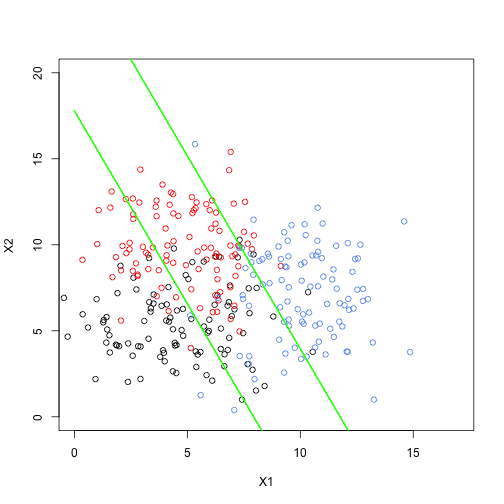
\includegraphics[width=.7\linewidth]{figure/linear-classifier} 

}

\caption[Three class simulated data seperated by linear regression]{Three class simulated data seperated by linear regression\label{fig:linear-classifier}}
\end{figure}


\end{knitrout}


Figure~\ref{fig:linear-classifier} shows our data point as well as the linear regression classifier. Here we try to seperate three classes with Linear regression. We simply set each classes value as 0, 1 and 2. And if response value less than 2/3, we believe it belongs to class 0; if it is larger than 2/3 but less than 4/3, that point belongs to class 1; if the response value is larger than 4/3, we put it into class 2.

There are several drawbacks for this methods. One of them is that we assumed all data should fall in to our plane and thus all possible points have response from 0 to 2, which is obviously not true. We might use Cross Validation to find the best seperate point (here is 2/3 and 4/3). Still, even though we can find different ways to improve linear regression method, it not regular to use linear regression to solve classification problem.

\subsection{KNN}
\label{knn}

\begin{knitrout}\tiny
\definecolor{shadecolor}{rgb}{0.969, 0.969, 0.969}\color{fgcolor}\begin{kframe}
\begin{alltt}
\hlstd{grid} \hlkwb{<-} \hlkwa{function}\hlstd{() \{}
    \hlstd{xx1} \hlkwb{<-} \hlkwd{seq}\hlstd{(}\hlnum{0}\hlstd{,} \hlnum{15}\hlstd{,} \hlkwc{length} \hlstd{=} \hlnum{1000}\hlstd{)}
    \hlstd{xx2} \hlkwb{<-} \hlkwd{seq}\hlstd{(}\hlnum{0}\hlstd{,} \hlnum{20}\hlstd{,} \hlkwc{length} \hlstd{=} \hlnum{1000}\hlstd{)}
    \hlstd{dat3} \hlkwb{<-} \hlkwd{matrix}\hlstd{(}\hlnum{0}\hlstd{,} \hlkwc{ncol} \hlstd{=} \hlnum{2}\hlstd{,} \hlkwc{nrow} \hlstd{=} \hlnum{1000} \hlopt{*} \hlnum{1000}\hlstd{)}
    \hlkwa{for} \hlstd{(i} \hlkwa{in} \hlnum{1}\hlopt{:}\hlnum{1000}\hlstd{) \{}
        \hlkwa{for} \hlstd{(j} \hlkwa{in} \hlnum{1}\hlopt{:}\hlnum{1000}\hlstd{) \{}
            \hlstd{dat3[j} \hlopt{+} \hlstd{i} \hlopt{*} \hlnum{1000} \hlopt{-} \hlnum{1000}\hlstd{,} \hlnum{1}\hlstd{]} \hlkwb{<-} \hlstd{xx1[i]}
            \hlstd{dat3[j} \hlopt{+} \hlstd{i} \hlopt{*} \hlnum{1000} \hlopt{-} \hlnum{1000}\hlstd{,} \hlnum{2}\hlstd{]} \hlkwb{<-} \hlstd{xx2[j]}
        \hlstd{\}}
    \hlstd{\}}
    \hlstd{mygrid} \hlkwb{<-} \hlkwd{data.frame}\hlstd{(dat3)}
\hlstd{\}}

\hlstd{NN} \hlkwb{<-} \hlkwa{function}\hlstd{() \{}
    \hlstd{Neighbors} \hlkwb{<<-} \hlkwd{rep}\hlstd{(}\hlnum{0}\hlstd{,} \hlkwd{nrow}\hlstd{(mygrid))}
    \hlkwa{for} \hlstd{(i} \hlkwa{in} \hlkwd{c}\hlstd{(}\hlnum{1}\hlopt{:}\hlkwd{nrow}\hlstd{(mygrid))) \{}
        \hlstd{distances} \hlkwb{<-} \hlstd{(mygrid}\hlopt{$}\hlstd{X1[i]} \hlopt{-} \hlstd{x1)}\hlopt{^}\hlnum{2} \hlopt{+} \hlstd{(mygrid}\hlopt{$}\hlstd{X2[i]} \hlopt{-} \hlstd{x2)}\hlopt{^}\hlnum{2}
        \hlstd{sort.distances} \hlkwb{<-} \hlkwd{sort.int}\hlstd{(distances,} \hlkwc{index.return} \hlstd{=} \hlnum{TRUE}\hlstd{)}
        \hlcom{# k=15}
        \hlkwa{if} \hlstd{((}\hlkwd{sum}\hlstd{(sort.distances}\hlopt{$}\hlstd{ix[}\hlnum{1}\hlopt{:}\hlnum{15}\hlstd{]} \hlopt{>} \hlnum{200}\hlstd{)}\hlopt{/}\hlnum{15}\hlstd{)} \hlopt{>} \hlnum{0.5}\hlstd{)}
            \hlstd{Neighbors[i]} \hlkwb{<-} \hlnum{3} \hlkwa{else if} \hlstd{((}\hlkwd{sum}\hlstd{(sort.distances}\hlopt{$}\hlstd{ix[}\hlnum{1}\hlopt{:}\hlnum{15}\hlstd{]} \hlopt{>} \hlnum{100}\hlstd{)}\hlopt{/}\hlnum{15}\hlstd{)} \hlopt{>} \hlnum{0.5}\hlstd{)}
            \hlstd{Neighbors[i]} \hlkwb{<-} \hlnum{2} \hlkwa{else} \hlstd{Neighbors[i]} \hlkwb{<-} \hlnum{1}
    \hlstd{\}}
    \hlstd{Neighbors} \hlkwb{<<-} \hlstd{Neighbors}
\hlstd{\}}

\hlstd{plotKNN} \hlkwb{<-} \hlkwa{function}\hlstd{() \{}
    \hlkwd{plot}\hlstd{(}\hlkwd{c}\hlstd{(}\hlnum{0}\hlstd{,} \hlnum{15}\hlstd{),} \hlkwd{c}\hlstd{(}\hlnum{0}\hlstd{,} \hlnum{20}\hlstd{),} \hlkwc{type} \hlstd{=} \hlstr{"n"}\hlstd{,} \hlkwc{xlab} \hlstd{=} \hlstr{"X1"}\hlstd{,} \hlkwc{ylab} \hlstd{=} \hlstr{"X2"}\hlstd{)}
    \hlkwd{points}\hlstd{(mygrid}\hlopt{$}\hlstd{X1[Neighbors} \hlopt{==} \hlnum{1}\hlstd{], mygrid}\hlopt{$}\hlstd{X2[Neighbors} \hlopt{==} \hlnum{1}\hlstd{],} \hlkwc{col} \hlstd{=} \hlstr{"skyblue"}\hlstd{)}
    \hlkwd{points}\hlstd{(mygrid}\hlopt{$}\hlstd{X1[Neighbors} \hlopt{==} \hlnum{2}\hlstd{], mygrid}\hlopt{$}\hlstd{X2[Neighbors} \hlopt{==} \hlnum{2}\hlstd{],} \hlkwc{col} \hlstd{=} \hlstr{"pink"}\hlstd{)}
    \hlcom{# points(mygrid$X1[Neighbors==3],mygrid$X2[Neighbors==3],col='green')}
    \hlkwd{points}\hlstd{(x1[}\hlnum{101}\hlopt{:}\hlnum{200}\hlstd{], x2[}\hlnum{101}\hlopt{:}\hlnum{200}\hlstd{],} \hlkwc{col} \hlstd{=} \hlstr{"RED"}\hlstd{,} \hlkwc{pch} \hlstd{=} \hlnum{20}\hlstd{)}
    \hlkwd{points}\hlstd{(x1[}\hlnum{1}\hlopt{:}\hlnum{100}\hlstd{], x2[}\hlnum{1}\hlopt{:}\hlnum{100}\hlstd{],} \hlkwc{col} \hlstd{=} \hlstr{"BLUE"}\hlstd{,} \hlkwc{pch} \hlstd{=} \hlnum{20}\hlstd{)}
    \hlkwd{points}\hlstd{(x1[}\hlnum{201}\hlopt{:}\hlnum{300}\hlstd{], x2[}\hlnum{201}\hlopt{:}\hlnum{300}\hlstd{],} \hlkwc{col} \hlstd{=} \hlstr{"black"}\hlstd{,} \hlkwc{pch} \hlstd{=} \hlnum{20}\hlstd{)}
\hlstd{\}}
\end{alltt}
\end{kframe}
\end{knitrout}

\begin{figure}
\centering
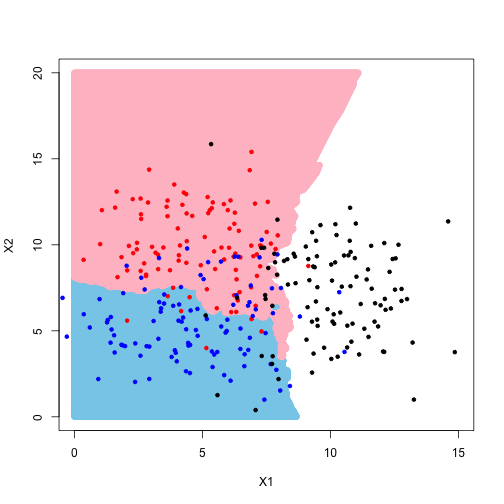
\includegraphics[width=.7\linewidth]{r-knn.png}
\caption{KNN Classifier with 3 classes}
\label{fig:knn}
\end{figure}

The KNN classifier is shown in Figure~\ref{fig:knn}. Instead of using knn funciton in package ``class'', we generate grid - a 1000000*2 Matrix - trying to cover every point in our plane. And by determining which class every point belongs to, we can obtain the KNN classifier boundry of our plane. If we want to draw that classifier line specifically, we can find the point whose at least two value of distance to class that calculated before are identical. Those point with identical distance consist of our KNN classifier.

\pagebreak
\subsection{Bayes Optimal Classifier}
\label{sec:bc}

\begin{knitrout}
\definecolor{shadecolor}{rgb}{0.969, 0.969, 0.969}\color{fgcolor}\begin{kframe}
\begin{alltt}
\hlstd{f1} \hlkwb{<-} \hlkwa{function}\hlstd{(}\hlkwc{x1}\hlstd{,} \hlkwc{x2}\hlstd{,} \hlkwc{mu1}\hlstd{,} \hlkwc{sigma1}\hlstd{,} \hlkwc{mu2}\hlstd{,} \hlkwc{sigma2}\hlstd{) \{}
    \hlstd{const1} \hlkwb{<-} \hlnum{1}\hlopt{/}\hlstd{(}\hlnum{2} \hlopt{*} \hlstd{pi} \hlopt{*} \hlstd{sigma1} \hlopt{*} \hlstd{sigma2)}
    \hlstd{f} \hlkwb{=} \hlkwd{exp}\hlstd{((}\hlopt{-}\hlstd{(x1} \hlopt{-} \hlstd{mu1)}\hlopt{^}\hlnum{2}\hlopt{/}\hlstd{sigma1}\hlopt{^}\hlnum{2} \hlopt{-} \hlstd{(x2} \hlopt{-} \hlstd{mu2)}\hlopt{^}\hlnum{2}\hlopt{/}\hlstd{sigma2}\hlopt{^}\hlnum{2}\hlstd{)}\hlopt{/}\hlnum{2}\hlstd{)} \hlopt{*} \hlstd{const1}
    \hlkwd{return}\hlstd{(f)}
\hlstd{\}}
\hlstd{BC} \hlkwb{<-} \hlkwa{function}\hlstd{() \{}
    \hlcom{# apply(a,1,which.max)}
    \hlstd{classifier} \hlkwb{<-} \hlkwd{matrix}\hlstd{(}\hlnum{0}\hlstd{,} \hlkwc{nrow} \hlstd{=} \hlkwd{nrow}\hlstd{(mygrid),} \hlkwc{ncol} \hlstd{=} \hlnum{3}\hlstd{)}
    \hlstd{classifier[,} \hlnum{1}\hlstd{]} \hlkwb{<-} \hlkwd{f1}\hlstd{(mygrid}\hlopt{$}\hlstd{X1, mygrid}\hlopt{$}\hlstd{X2,} \hlkwc{mu1} \hlstd{=} \hlnum{5}\hlstd{,} \hlkwc{sigma1} \hlstd{=} \hlnum{2.5}\hlstd{,} \hlkwc{mu2} \hlstd{=} \hlnum{5}\hlstd{,}
        \hlkwc{sigma2} \hlstd{=} \hlnum{2}\hlstd{)}
    \hlstd{classifier[,} \hlnum{2}\hlstd{]} \hlkwb{<-} \hlkwd{f1}\hlstd{(mygrid}\hlopt{$}\hlstd{X1, mygrid}\hlopt{$}\hlstd{X2,} \hlkwc{mu1} \hlstd{=} \hlnum{5}\hlstd{,} \hlkwc{sigma1} \hlstd{=} \hlnum{2}\hlstd{,} \hlkwc{mu2} \hlstd{=} \hlnum{10}\hlstd{,}
        \hlkwc{sigma2} \hlstd{=} \hlnum{2}\hlstd{)}
    \hlstd{classifier[,} \hlnum{3}\hlstd{]} \hlkwb{<-} \hlkwd{f1}\hlstd{(mygrid}\hlopt{$}\hlstd{X1, mygrid}\hlopt{$}\hlstd{X2,} \hlkwc{mu1} \hlstd{=} \hlnum{10}\hlstd{,} \hlkwc{sigma1} \hlstd{=} \hlnum{2}\hlstd{,} \hlkwc{mu2} \hlstd{=} \hlnum{7}\hlstd{,}
        \hlkwc{sigma2} \hlstd{=} \hlnum{2.5}\hlstd{)}
    \hlstd{classifier1} \hlkwb{<-} \hlkwd{apply}\hlstd{(classifier,} \hlnum{1}\hlstd{, which.max)}

\hlstd{\}}
\hlstd{plotBC} \hlkwb{<-} \hlkwa{function}\hlstd{() \{}
    \hlkwd{plot}\hlstd{(}\hlkwd{c}\hlstd{(}\hlnum{0}\hlstd{,} \hlnum{15}\hlstd{),} \hlkwd{c}\hlstd{(}\hlnum{0}\hlstd{,} \hlnum{20}\hlstd{),} \hlkwc{type} \hlstd{=} \hlstr{"n"}\hlstd{,} \hlkwc{xlab} \hlstd{=} \hlstr{"X1"}\hlstd{,} \hlkwc{ylab} \hlstd{=} \hlstr{"X2"}\hlstd{)}
    \hlkwd{points}\hlstd{(mygrid}\hlopt{$}\hlstd{X1[classifier1} \hlopt{==} \hlnum{1}\hlstd{], mygrid}\hlopt{$}\hlstd{X2[classifier1} \hlopt{==} \hlnum{1}\hlstd{],} \hlkwc{col} \hlstd{=} \hlstr{"skyblue"}\hlstd{)}
    \hlkwd{points}\hlstd{(mygrid}\hlopt{$}\hlstd{X1[classifier1} \hlopt{==} \hlnum{2}\hlstd{], mygrid}\hlopt{$}\hlstd{X2[classifier1} \hlopt{==} \hlnum{2}\hlstd{],} \hlkwc{col} \hlstd{=} \hlstr{"pink"}\hlstd{)}
    \hlkwd{points}\hlstd{(mygrid}\hlopt{$}\hlstd{X1[classifier1} \hlopt{==} \hlnum{3}\hlstd{], mygrid}\hlopt{$}\hlstd{X2[classifier1} \hlopt{==} \hlnum{3}\hlstd{],} \hlkwc{col} \hlstd{=} \hlstr{"grey"}\hlstd{)}
    \hlkwd{points}\hlstd{(x1[}\hlnum{101}\hlopt{:}\hlnum{200}\hlstd{], x2[}\hlnum{101}\hlopt{:}\hlnum{200}\hlstd{],} \hlkwc{col} \hlstd{=} \hlstr{"RED"}\hlstd{,} \hlkwc{pch} \hlstd{=} \hlnum{20}\hlstd{)}
    \hlkwd{points}\hlstd{(x1[}\hlnum{1}\hlopt{:}\hlnum{100}\hlstd{], x2[}\hlnum{1}\hlopt{:}\hlnum{100}\hlstd{],} \hlkwc{col} \hlstd{=} \hlstr{"BLUE"}\hlstd{,} \hlkwc{pch} \hlstd{=} \hlnum{20}\hlstd{)}
    \hlkwd{points}\hlstd{(x1[}\hlnum{201}\hlopt{:}\hlnum{300}\hlstd{], x2[}\hlnum{201}\hlopt{:}\hlnum{300}\hlstd{],} \hlkwc{col} \hlstd{=} \hlstr{"black"}\hlstd{,} \hlkwc{pch} \hlstd{=} \hlnum{20}\hlstd{)}
\hlstd{\}}
\end{alltt}
\end{kframe}
\end{knitrout}

\begin{figure}[ht]
\centering
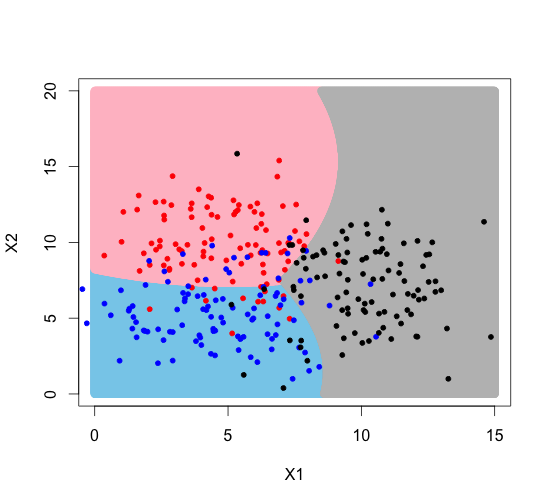
\includegraphics[width=.7\linewidth]{bc.png}
\caption{Bayes Optimal Classifier for 3 classes}
\label{fig:bc}
\end{figure}


The Figure~\ref{fig:bc} one Page~\pageref{fig:bc} shows the Optimal Bayes Classifier. Here we use the same strategy as KNN. Since we have the exact density function of all three data set, we can calculate probability of every points form ``mygrid'' for each category. And then we can simply compare three probabilities for each point and determine which class it belongs to (belongs to class that has highest probability).


\end{document}
